
\section{Getting started}\label{sect:start}\index{PISM!getting started}

In this section we give an extended example applying PISM to the Greenland ice sheet.  We use recent data sets provided by the \href{http://websrv.cs.umt.edu/isis/index.php/SeaRISE_Assessment}{Sea-level Response to Ice Sheet Evolution (SeaRISE)}) group.  SeaRISE is a community-organized assessment process to provide an upper bound of ice sheet contributions to sea level in the next 100--200 years, especially for the next IPCC report in 2013.

The example in this section is a quick, hands-on first look at PISM.  It is not an in-depth tutorial, and many details of what is happening will only be explained later.  The sections on the older EISMINT-Greenland and EISMINT-Ross modeling cases, for instance, do a more complete job of explaining the ways users will need to preprocess not-so-clean input data and then make, and evaluate, modeling choices.

The PISM output figures in this section were produced using a supercomputer.  However, in order for the examples here to run on a typical workstation, a rather coarse $20\,\textrm{km}$ grid is used.  One purpose of PISM is to make much higher spatial resolution actually possible, but it does indeed require large-scale \emph{parallel} processing.


\subsection{Install PISM}

See the \emph{Installation Manual}
   \begin{center}
     \href{http://www.pism-docs.org/dev/pdfs/installation-dev.pdf}{\t{www.pism-docs.org/dev/pdfs/installation-dev.pdf}}
   \end{center}
to install PISM.  Once installed, executables \verb|pismr| and \verb|pclimate|, and several others, will be in the \verb|bin| subdirectory of the main PISM directory.  The main PISM directory might be at \verb|/home/username/pism-dev/|, for example.  The instructions below assume you start from that main PISM directory.  We also assume you are using a \verb|bash| shell or at least one that accepts \verb|bash| syntax.


\subsection{Obtain and preprocess the input data}

The NetCDF data file which we use for input is freely-available online.  Descriptions of the data it contains, and a link to the file itself, are on this web page: 
\medskip

\centerline{\protect{\textbf{\url{http://websrv.cs.umt.edu/isis/index.php/Present_Day_Greenland}}}}
\medskip

\noindent The quickest way to get the file itself is to do

\verb|$ cd examples/searise-greenland|

\verb|$ ./preprocess.sh|

\noindent The script \verb|preprocess.sh|\footnote{\protect{This script requires \texttt{wget} and NCO (NetCDF Operators; \url{http://nco.sourceforge.net/})}.} downloads the ``master'' present-day data set and adjusts it to make it PISM-readable.\footnote{The script looks for \texttt{Greenland\_5km\_v0.93.nc}.  If a different version number is desired, edit the script to change the line ``\texttt{DATAVERSION=0.93}''.}

Preprocessing creates three NetCDF files from the master data, each of which has small ``metadata'' changes so that they can be read by PISM.  These metadata can be listed at the command line, or put in a text file, by \verb|ncdump -h|.  Two of the new files contain famous time-dependent paleo-climate records from ice core (\verb|pism_dT.nc| has GRIP) and seabed core records (\verb|pism_dSL.nc| has SPECMAP).

Any of these NetCDF files can be viewed with \verb|ncview| or other NetCDF visualization tools.  (See Table \ref{tab:NetCDFview} below.)  Application of \verb|pyNGL| tools to \verb|Greenland_5km_v0.93.nc| produced figures \ref{fig:sr-input1} and  \ref{fig:sr-input2}, for example.

\begin{figure}[ht]
\centering
\mbox{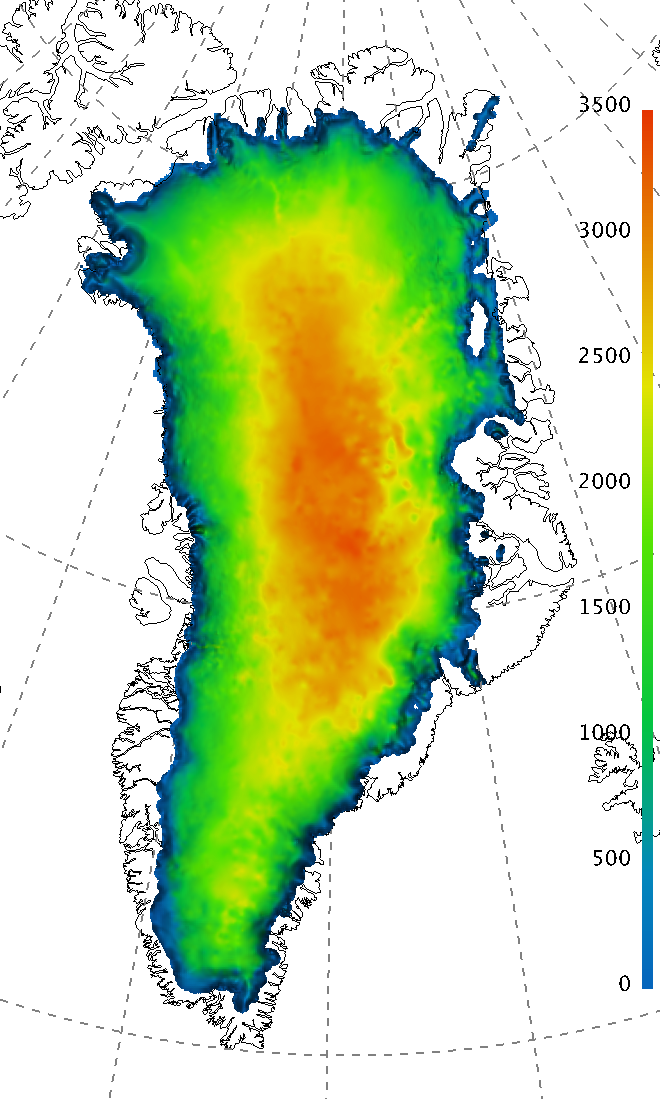
\includegraphics[width=2.5in,keepaspectratio=true]{sr-greenland-thk}
 \qquad\qquad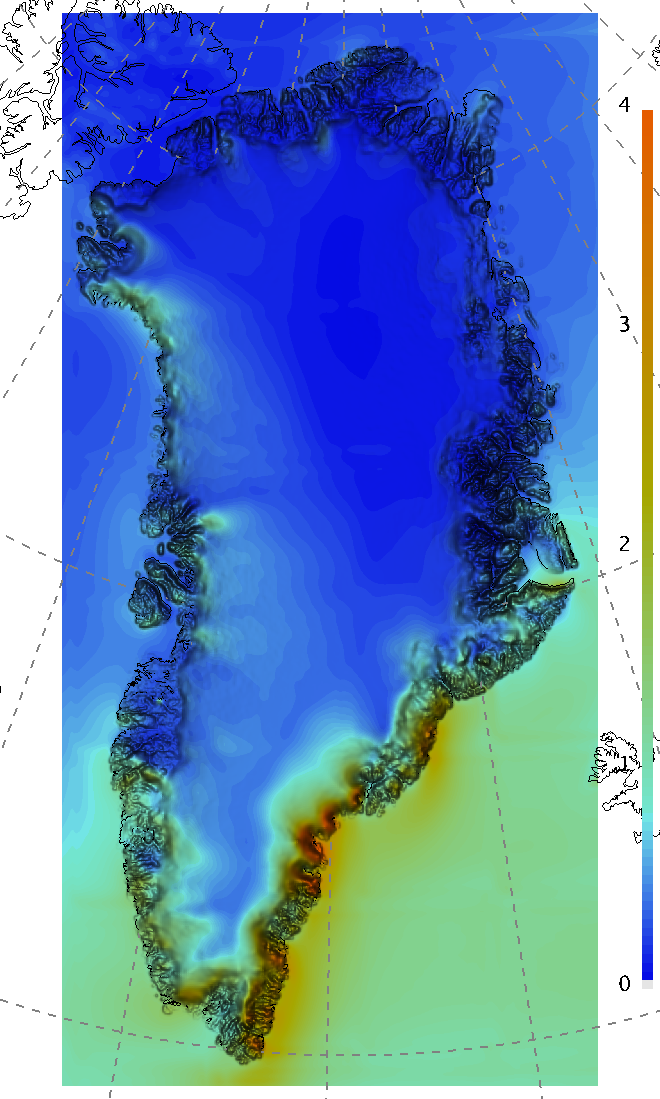
\includegraphics[width=2.5in,keepaspectratio=true]{sr-greenland-prcp}}
\caption{The input present-day ice thickness (left; m) and present-day precipitation (right; m $\text{a}^{-1}$ ice equivalent) for SeaRISE-Greenland.  Figures produced with IDV}
\label{fig:sr-input1}
\end{figure}

\begin{figure}[ht]
\centering
\mbox{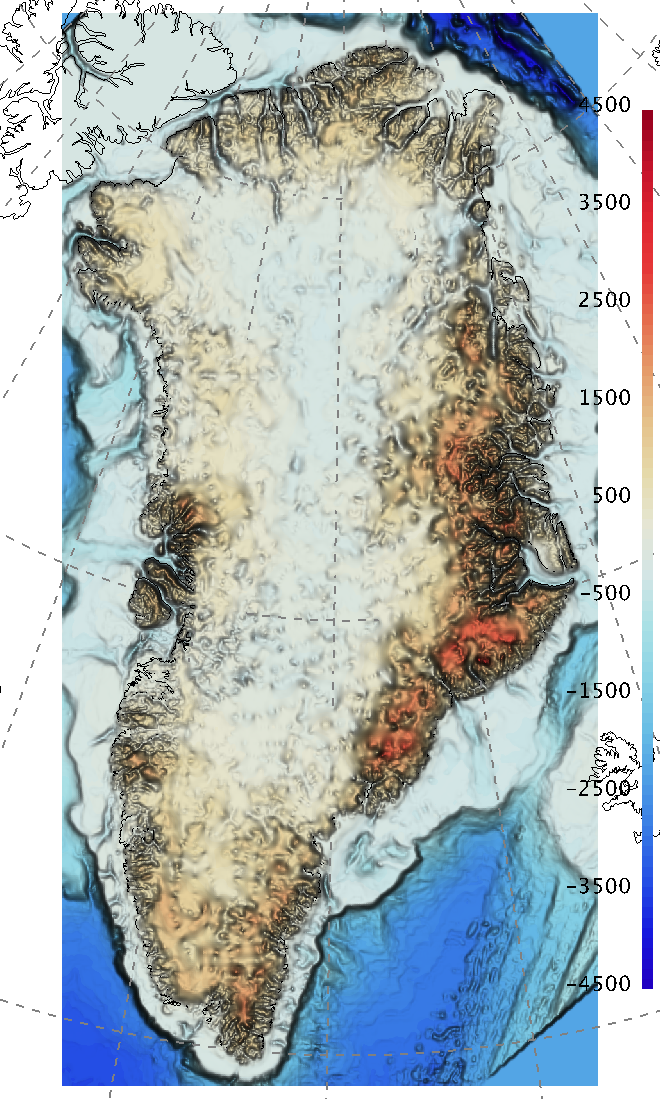
\includegraphics[width=2.5in,keepaspectratio=true]{sr-greenland-topg}
 \qquad\quad 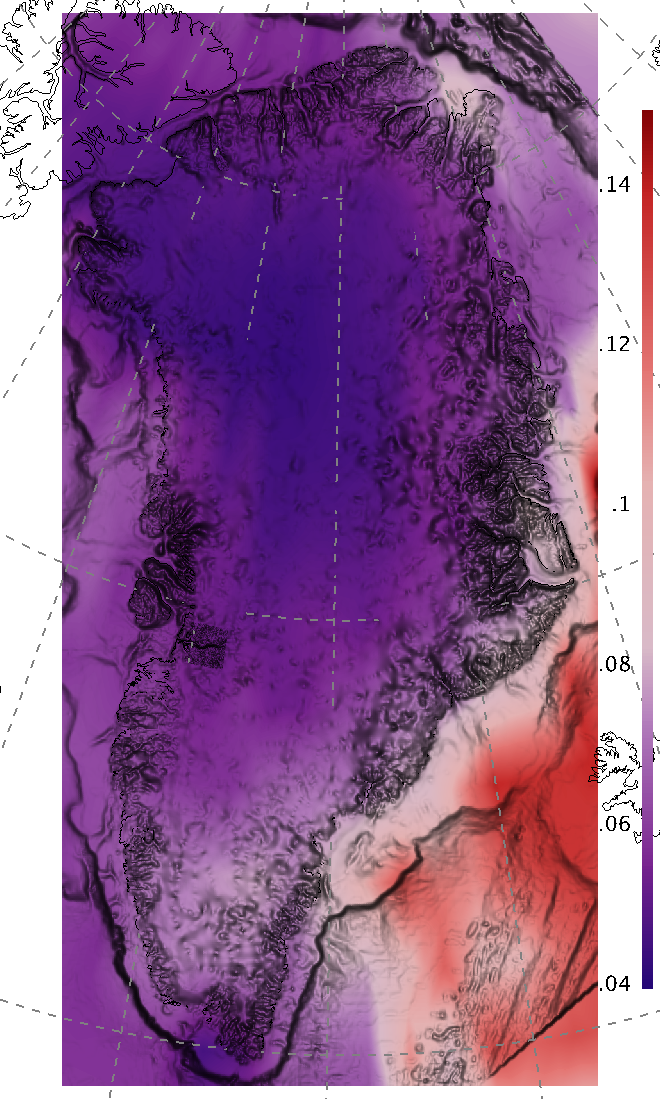
\includegraphics[width=2.5in,keepaspectratio=true]{sr-greenland-bheatflx}}
\caption{The input bedrock elevation (left; m) and geothermal flux (right; W $\text{m}^{-2}$) for SeaRISE-Greenland.  Figures produced with IDV}
\label{fig:sr-input2}
\end{figure}


\subsection{Run PISM}

We are ready to run PISM, but, perhaps even more than many unix programs, PISM allows \emph{a lot} of command-line options.  Furthermore there are configuration parameters that get read from a file, namely in \verb|lib/pism_config.nc|.  Because it is an ice flow simulation program designed to handle many different ice sheet, shelve, and glacier configurations, the list of user-configurable flags and parameters is quite long.  For a complete list see
\begin{center}
\url{http://www.pism-docs.org/dev/doxy/html/config.html}
\end{center}

These many options and parameters imply that one should often build a \emph{script} to run PISM with the correct options.  We have done this for SeaRISE-Greenland.  Also, as explained in the rest of this \emph{User's Manual}, modeling ice sheets requires the integration of paleo-climatic and long-time-scale information into the model state, so our script is called ``\verb|spinup.sh|''.  The spin-up stage is the one which generally requires the most processor-hours, compared to a ``forecast'' stage.

To see what the run involves, do this:

\verb|$ PISM_DO=echo|

\verb|$ ./spinup.sh|

\noindent Setting the environment variable \verb|PISM_DO| in this way tells \verb|spinup.sh| just to print out the commands it is about to run, not do them.  Note that ``\verb|mpiexec -n 2 pismr|'' appears in the PISM runs done by \verb|spinup.sh|.  This means that the PISM executable \verb|pismr| is run in parallel on two processes (e.g.~cores).  The executable name ``\verb|pismr|'' stands for the standard ``run'' mode of PISM, in contrast to other, specialized run modes described later.

For the rest of this example, we assume you have a workstation with 8 cores, which is typical of 2010 resources.

The script \verb|spinup.sh| starts by ``bootstrapping.''  This term describes the creation, by heuristics and simplified models, of the kind of full initial conditions needed for the evolving, time-dependent model.  Specifically, the first 100 model year run with 8 processes will look like this (\emph{no need to type here \dots patience \dots}):
\small
\begin{verbatim}
  mpiexec -n 8 pismr -ocean_kill -eta -skip 2 -boot_from pism_Greenland_5km_v0.93.nc \
    -Mx 76 -My 141 -Lz 4000 -Lbz 2000 -Mz 41 -Mbz 16 \
    -atmosphere searise_greenland -surface pdd -pdd_fausto \
    -y 100 -o g20km_pre100.nc
\end{verbatim}
\normalsize
The options describe a $76\times 141$ point grid in the horizontal, which gives 20 km grid spacing in both directions.  There are also important choices about the vertical extent and resolution of the computational domain; more on those later.  

Now, instead of typing-in the above PISM command with all its options, however, get the run going by

\verb|$ export PISM_DO=|

\verb|$ ./spinup.sh 8 >> out.spin20km &|

\noindent PISM will show what it is doing in the text file \verb|out.spin20km| while it runs in the background.  Using \verb|less| is a good way to watch a growing text file.  The run will fairly quickly---within a minute---produce a very-early flow result in \verb|g20km_pre100.nc| and soon after that a boundary conditions sample result \verb|g20km_climate-500a.nc|.  The latter is effectively a movie of the stored climatic inputs to the Greenland ice sheet model, plus the results from surface models, especially for surface mass balance, but all assuming steady geometry.  Such a result is important to look at early in the modeling process because surface mass balance and surface temperature are (and must) be simulated for this kind of spinup.

The total run time for the complete 20km spinup, which models 125,000 model years with ``full physics'' of the polythermal SIA+SSA hybrid type (section \ref{sect:dynamics}) uses about 60 processor-hours.  If done without membrane stresses (SIA only) this time would be greatly reduced.  The polythermal (vs ``cold'') physics choice has no performance disadvantage (again, section \ref{sect:dynamics}).

The next paragraphs describes what happens and what files are produced.  We believe that the modeling choices represented here are reasonable choices, but there is certainly no claim that this is the ``only way to do it''.  The user is encouraged to try other versions and experiment; that is the point of a model!

After the completion of the first 100 model year run, the one giving \verb|g20km_pre100.nc| as output, we start a run to generate a more credible enthalpy (thus temperature) field in which the modeled ice internal energy, its softness, its flow velocity, its stored basal water, and its basal melt rate are all in better balance with the the ice sheet geometry.  In particular the upper and lower surfaces of this ice are held fixed; the former is held fixed by the option \intextoption{no_mass} while the latter is held fixed because we do not apply a bed deformation model at this stage.\footnote{Thus the resulting enthalpy field is in approximate equilibrium with a velocity field for which the surface kinematical equation \cite{Fowler} is \emph{not} satisfied.}  There is no sliding at this stage.  We sometimes call this stage ``pre-spinup''; in any case it follows on ``bootstrapping'' and comes before ``actual spinup'' which uses the paleo-climatic record.  This ``pre-spinup'' stage goes for 50000 model years and yields the file \verb|g20km_steady.nc| at the end.  Along the way the file \verb|ex_g20km_steady.nc| is updated at every 500 model years, and it can be used to evaluate the degree to which we have reached a thermomechanically-coupled steady state.

Before we proceed with the actual spinup and its paleo-climate forcing, we add another short smoothing run which produces \verb|g20km_SIA.nc| after 100 model years.  This state has approximate thermomechanical equilibrium and has a surface geometry which is close to the present-day one but satisfies the surface kinematical equation.

The resulting model state in \verb|g20km_SIA.nc| is our model for the state of the Greenland ice sheet at time of the beginning of the paleo-climate data provided in the SeaRISE data set, namely 125,000 B.P.  Two views of this state are in Figure \ref{fig:sr-spinstart}.

\begin{figure}[ht]
\centering
FIXME: add temppabase from end of ex_g20km_steady.nc and driving stress taud from g20km_SIA.nc
\caption{The pressure-adjusted basal temperature (left) and driving stress (right) at the beginning of the paleo-climate-driven spinup stage.  Figures produced with ncview}
\label{fig:sr-spinstart}
\end{figure}



FIXME





\subsection{Handling NetCDF files}\label{subsect:nctoolsintro}  At a superficial level, PISM is just a program which takes one or more NetCDF files as input, does some computation, and produces one or more NetCDF files as output.  As a result, the user must and extract some meaning from the NetCDF output files and also, in the general case, use other tools to create NetCDF files for input to PISM.\footnote{Regarding the creation of input files, see the section \ref{sec:bootstrapping-format} and table \ref{tab:modelhierarchy} for ideas about the data necessary for modeling.}

The most basic tools for converting NetCDF files to and from a standard text representation are called \verb|ncdump| and \verb|ncgen|.  A glance at Unix \verb|man| pages for these tools might be wise at this time.

We most-regularly use \verb|ncview| to look at NetCDF files.  Table \ref{tab:NetCDFview} lists NetCDF tools that can be useful for for visualizing and post-processing PISM output files, and for preparing input data.  We find \texttt{ncview}, NCO, IDV and PyNGL especially useful.

\newcommand{\netcdftool}[1]{#1\index{NetCDF!tools!#1}}
\begin{table}[ht]
\centering
\caption{Some tools for viewing and modifying NetCDF files.}\label{tab:NetCDFview} 
\small
\begin{tabular}{llp{0.4\linewidth}}
  \\\toprule
  \textbf{Tool} & \textbf{Site} & \textbf{Function}\\ \midrule
\netcdftool{\texttt{ncdump}} & \emph{included with any NetCDF distribution} & dump binary NetCDF as \texttt{.cdl} (text) file \\
\netcdftool{\texttt{ncgen}} & \emph{included with any NetCDF distribution} & convert \texttt{.cdl} file to binary NetCDF \\
\netcdftool{\texttt{ncview}} & \href{http://meteora.ucsd.edu/~pierce/ncview_home_page.html}{\texttt{meteora.ucsd.edu/$\sim$pierce}} & quick graphical view \\
\netcdftool{IDV} & \href{http://www.unidata.ucar.edu/software/idv/}{\t{www.unidata.ucar.edu/software/idv/}} & more complete visualization \\
%\netcdftool{Paraview} & \href{http://www.paraview.org}{\t{www.paraview.org}} & powerful open-source parallel visualization \\
%\netcdftool{NCL} &  \href{http://www.ncl.ucar.edu}{\t{www.ncl.ucar.edu}} & NCAR Command Language, open-source\\
\netcdftool{PyNGL} &  \href{http://www.pyngl.ucar.edu}{\t{www.pyngl.ucar.edu}} & Python version of NCL, open-source\\
%\netcdftool{VisIt} & \href{http://visit.llnl.gov}{\t{visit.llnl.gov}} & advanced parallel visualization \\
\netcdftool{NCO}\index{NCO (NetCDF Operators)} & \href{http://nco.sourceforge.net/}{\t{nco.sourceforge.net/}} & ``NetCDF Operators'': manipulations at command line\\
\netcdftool{CDO} & \href{http://www.mpimet.mpg.de/fileadmin/software/cdo/}{\texttt{www.mpimet.mpg.de/fileadmin/software/cdo/}} & Climate Data Operators (a set of command-line tools)
\\\bottomrule
\end{tabular}
\normalsize
\end{table}

This website gives additional NetCDF-related tools:

\centerline{ \url{http://www.unidata.ucar.edu/software/netcdf/docs/software.html} } 


%%% Local Variables: 
%%% mode: latex
%%% TeX-master: "manual"
%%% End: 

